\section{Call parameters and consumption}\label{sec:usage_modality}
In this section, we analyze the impact of different usage modalities such as the number of persons in the call, viewing mode, and device type on the network consumption. 
\subsection{Number of Users}
We fix the viewing mode in gallery, where no one user's video is pinned. We find that increasing the number of participants may reduce the network utilization. In particular, the sending rate decreases as the number of participants increases. One reason for this is that increasing the number of participants in a call reduces the size of their video on the receiver's screen. As a result, the sender's video resolution can decrease. Similarly, we see how the received bitrate drops dramatically at 5 and 7 participants for Zoom and Meet, respectively. We observe that Teams is also exhibiting a downward trend at 8 participants. 
\begin{figure}[]
    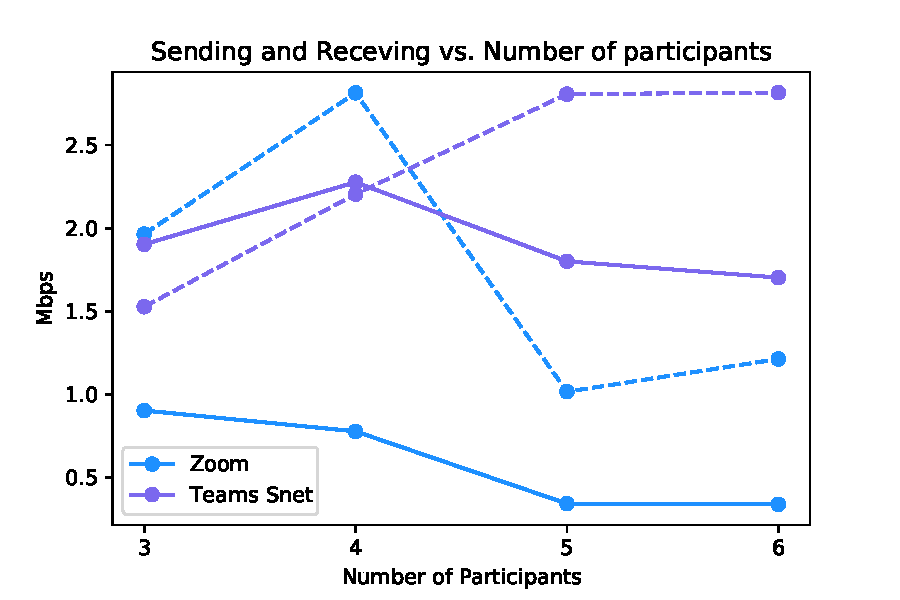
\includegraphics[width=0.35\textwidth,keepaspectratio]{../figures/modality/sending_call.pdf}
    \caption{Sending and Receiving Rate vs. Num Participants}
    \label{fig:loss_latency}
\end{figure}

\subsection{Viewing Mode}
\begin{figure}[]
    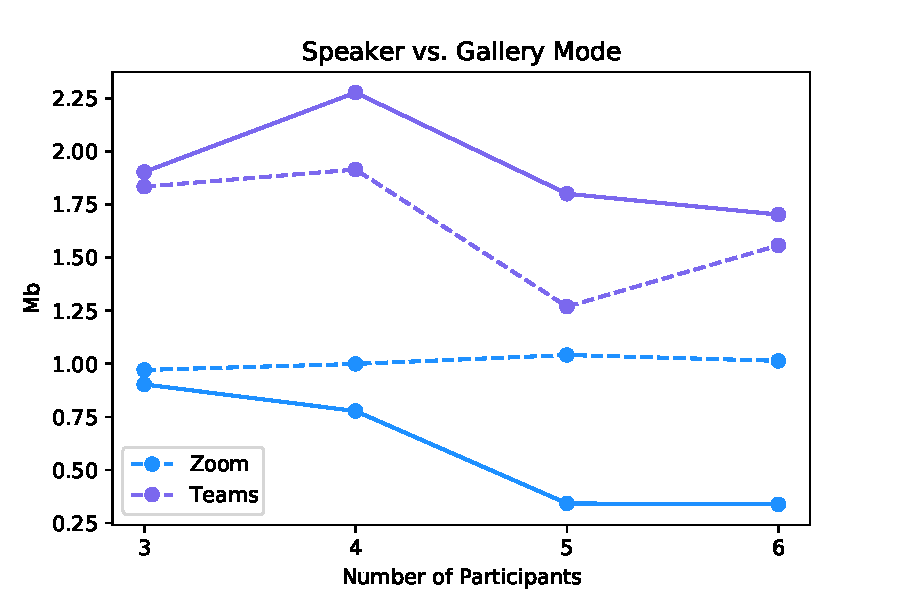
\includegraphics[width=0.35\textwidth,keepaspectratio]{../figures/modality/call_modality.pdf}
    \caption{Speaker vs. Gallery Mode}
    \label{fig:loss_latency}
\end{figure}
We find that viewing a user's video in speaker mode leads to greater network consumption on the user's network. When C1's video is pinned, all other clients view a higher resolution from video. Thus, C1 must continue sending at a higher resolution. Zoom consistently sends at 1 Mbps when all clients pin C1's video, regardless of the number of participants. 
\begin{figure}[]
    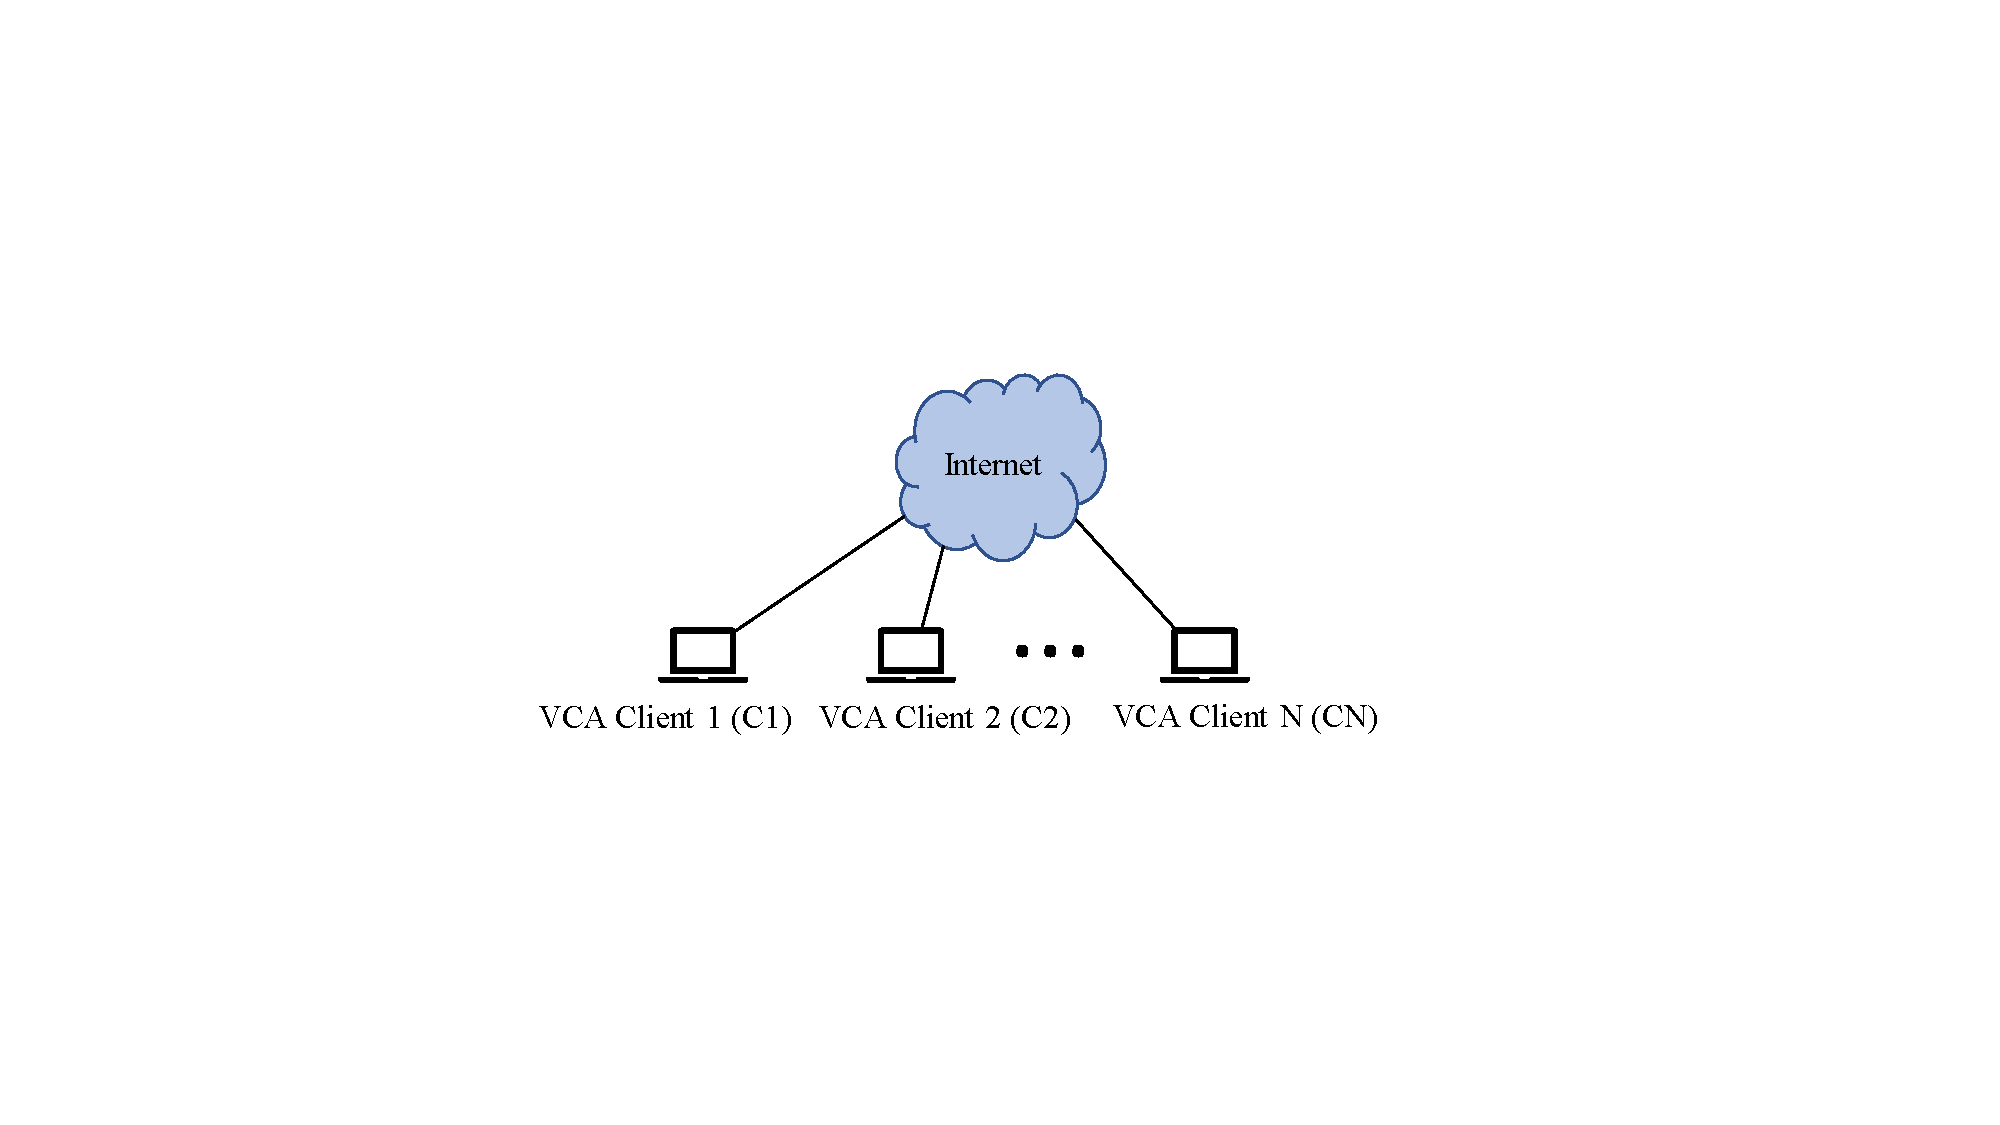
\includegraphics[width=0.35\textwidth,keepaspectratio]{../figures/methodology/modality-setup.pdf}
    \caption{Modality Setup}
    \label{fig:loss_latency}
\end{figure}